      
               
                \begin{ledgroupsized}[r]{120mm}
                \footnotesize 
                \pstart                
                \noindent\textbf{\"{U}berlieferung:}   
                \pend
                \end{ledgroupsized}
            
              
                            \begin{ledgroupsized}[r]{114mm}
                            \footnotesize 
                            \pstart \parindent -6mm
                            \makebox[6mm][l]{\textit{L}}Konzept: LH XXXV 14, 2 Bl. 129\textendash134. 3 Bog. 2\textsuperscript{o}. 5 S. Textfolge: Bl. 134 v\textsuperscript{o}, Bl. 129 r\textsuperscript{o}, Bl. 133 v\textsuperscript{o}, Bl. 132 r\textsuperscript{o}, Bl. 131 v\textsuperscript{o}. Bl. 129 v\textsuperscript{o}, Bl. 131 r\textsuperscript{o}, Bl. 132 v\textsuperscript{o}, Bl. 133 r\textsuperscript{o}, Bl. 134 r\textsuperscript{o} sowie Bl. 130 leer. Fortsetzung des Textes am Ende von Bl. 131 v\textsuperscript{o} durch 11 Zeilen am linken unteren Rand. Daran anschließend 6 Zeilen am linken Rand quer geschrieben.\\Cc 2, Nr. 475 \pend
                            \end{ledgroupsized}
                %\normalsize
                \vspace*{5mm}
                \begin{ledgroup}
                \footnotesize 
                \pstart
            \noindent\footnotesize{\textbf{Datierungsgr\"{u}nde}: Wir datieren das St\"{u}ck nach dem Wasserzeichen, das sich auch auf den Texttr\"{a}gern der Exzerpte aus O. v. Guerickes \cite{00055}\textit{Experimenta nova} findet.}
                \pend
                \end{ledgroup}
            
                \vspace*{8mm}
                \pstart 
                \normalsize
            [134 v\textsuperscript{o}] \selectlanguage{italian}\textit{Saggi di naturali Esperienze fatte nell'Accademia del Cimento sotto la protettione del Serenissimo principe Leopoldo}\protect\index{Namensregister}{\textso{Leopoldo de Medici} 1617\textendash 1675} \textit{di Toscana, e descritte dal Secretario di essa Accademia}\selectlanguage{latin} devise in frontispicio, aurum in Camino, cum inscriptione  provando e riprovando in Fiorenze\protect\index{Ortsregister}{Florenz (Fiorenze, Florentia)} per Giuseppe Cocchini\protect\index{Namensregister}{\textso{Cocchini}, Giuseppe}  al insigne della Stella 1667. Al Serenissimo Ferdinando II. Gran Duca di Toscana\protect\index{Namensregister}{\textso{Toscana: Ferdinand II.}, Großherzog der Toscana 1628\textendash 1670}.\pend \pstart \textso{Exper. Florent.} praef. Academia instituta 1657.\pend \pstart \textso{Dichiaratione delle instrumenti del caldo e freddo, fig. 1.}\edtext{}{\lemma{\textso{1.}}\Bfootnote{\textsc{L. Magalotti, }\cite{00143}\textit{Saggi di naturali esperienze}, Florenz 1667, S.~III.}}  ibi ait a vitri flatore formandam pilam\protect\index{Sachverzeichnis}{pila} cum canali, ita comparatam, ut repleta spiritu vini\protect\index{Sachverzeichnis}{spiritus!vini} ad certum colli signum, simplex  frigus aut glaciei non sufficiat ad condensandam infra 20 gradum  canalis, nec summus calor aestatis \edtext{ferventissimae}{\lemma{}\Afootnote{ferventissimae \textit{ erg.} \textit{ L}}} sufficiat ad extendendam  ultra gradum 80.\edtext{}{\lemma{80.}\Bfootnote{\textsc{L. Magalotti, }\cite{00143}a.a.O., S.~IV.}} Sed quia difficile plane evacuare rectius  erit fortasse, canalem esse summae subtilitatis. Habent Thermometrum\protect\index{Sachverzeichnis}{thermometrum} fig. 4. (pag. 9.)\edtext{}{\lemma{9.)}\Bfootnote{\cite{00143}\textsc{L. Magalotti}, a.a.O., S.~IX.}} intortum, sed hoc propter  nullam aliam rationem, quam quia idem longissime productum  pondere suo frangeretur. Nihil ergo hoc ad Barometrum\protect\index{Sachverzeichnis}{barometrum}  meum spirale.\pend\clearpage \pstart Declaratio Hygrometri\protect\index{Sachverzeichnis}{hygrometrum}.\edtext{}{\lemma{Hygrometri.}\Bfootnote{\cite{00143}\textsc{L. Magalotti}, a.a.O., S.~XII.}} Sumitur Truncus coni ex saccaro,  intus cavus et pice obductus, extra sopponato di latta,  acumine deorsum vergente, inseritur in similem conum vitrum,  impletur intus nive, aut glacie minutissime trita. Humidum  aeris subtilissimum frigori vitri paulatim adhaerebit, primumque  instar subtilissimae telae velabit, post in guttas formabitur  in Cylindrum suppositum in gradus divisum distillantes, et pendulo\protect\index{Sachverzeichnis}{pendulum}  notabitur, quanto tempore quantum aquae sic paretur. Id enim  determinabit gradus humiditatis. Inde et determinabimus qui venti  magis humidi vel sicci.\pend \pstart \textso{De Chronometro.}\protect\index{Sachverzeichnis}{chronometrum} Palam penduli\protect\index{Sachverzeichnis}{pendulum} ex duobus filis  suspendunt ne in
            \begin{wrapfigure}{l}{0.3\textwidth}                    
         \begin{center}
                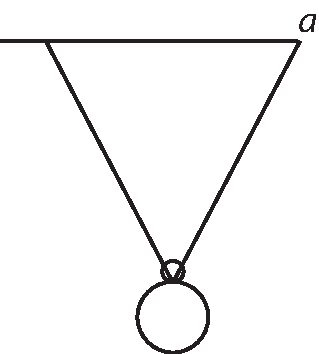
\includegraphics[width=0.3\textwidth]{images/35_14_2_134v}\\\textit{[Fig. 1]} 
                        %\caption{Bildbeschreibung}
                        \end{center}
                        \end{wrapfigure}
               spiras se circa filum intorquere  et gyrare potius quam vibrare possit. Idque utile est etiam  ad attrahendum facile laxandumque filum, attrahitur  enim saltem in uno loco ut in \textit{a}\edtext{}{\lemma{in}\Bfootnote{\cite{00143}\textsc{L. Magalotti}, a.a.O., S.~XVII.}} pila\protect\index{Sachverzeichnis}{pila} nihilominus semper in infimum  locum descendere vibrationes frequentiores intra idem tempus  quanto brevius filum. Galilaeus\protect\index{Namensregister}{\textso{Galilei} (Galilaeus, Galileus), Galileo 1564\textendash 1642} qui primus jam  anno 1583. observavit vibrationes pendulorum\protect\index{Sachverzeichnis}{vibratio penduli} esse proxime aequidiuturnas observavit inquam non \edtext{omnes vibrationes fieri}{\lemma{non}\Afootnote{ \textit{ (1) }\ omnia pendula\protect\index{Sachverzeichnis}{pendulum|textit} moveri \textit{ (2) }\ omnes vibrationes fieri \textit{ L}}} in temporibus  praecise inter se aequalibus. Nam quae quieti propiores eas breviori  tempore absolvi quam primas, ut dicetur suo loco.\edtext{}{\lemma{loco.}\Bfootnote{\cite{00143}\textsc{L. Magalotti}, a.a.O., S.~XX.}} Et repetitis vibrationibus differentia tandem reditur sensibilis. Primus omnium Galilaeus\protect\index{Namensregister}{\textso{Galilei} (Galilaeus, Galileus), Galileo 1564\textendash 1642} cogitavit de pendulis\protect\index{Sachverzeichnis}{pendulum} ad Horologium\protect\index{Sachverzeichnis}{horologium} applicandis, quod anno 1649. filius ejus Vincentius\protect\index{Namensregister}{\textso{Galilei} (Galilaeus), Vincenzio 1606\textendash 1649} Galilaei \protect\index{Namensregister}{\textso{Galilei} (Galilaeus, Galileus), Galileo 1564\textendash 1642} executus est,\edtext{}{\lemma{est,}\Bfootnote{\cite{00143}\textsc{L. Magalotti}, a.a.O., S.~XXII.}} ibi enim pendulum\protect\index{Sachverzeichnis}{pendulum} viribus Elaterii\protect\index{Sachverzeichnis}{elaterium} vel ponderis cogitur ex eadem semper altitudine labi. Habebat pendulum\protect\index{Sachverzeichnis}{vibratio penduli} quod absolvevat vibrationem in dimidio horae minuto secundo. Breviores tam velociter vibrant, ut oculi sequi non possint.\pend 
               \pstart \textso{De pressione Aeris.}\protect\index{Sachverzeichnis}{pressio!aeris} Primus Torricelli\protect\index{Namensregister}{\textso{Torricelli} (Torricellius), Evangelista 1608\textendash 1647} anno 1643. invento  experimento Hydrargyri\protect\index{Sachverzeichnis}{hydrargyrus} credidit aeris pressionem\protect\index{Sachverzeichnis}{pressio!aeris} esse in causa.\edtext{}{\lemma{causa.}\Bfootnote{\cite{00143}\textsc{L. Magalotti}, a.a.O., S.~XXIII.}} Aqua  in vacuum Torricellianum\protect\index{Sachverzeichnis}{vacuum!Torricellianum} attrahi potest ex altitudine \selectlanguage{italian}\textit{di braccia  diciassette e mezzo}\selectlanguage{latin}\edtext{}{\lemma{\textit{mezzo}}\Bfootnote{\cite{00143}\textsc{L. Magalotti}, a.a.O., S.~XXVIII.}} in circa, idem aer sustinet brachium et dimidium circiter argenti vivi\protect\index{Sachverzeichnis}{argentum!vivum}